% !TEX root = ./main.tex

\chapter{Parallel Pathway: Simultaneous Localization and Caption Generation}
\label{chap:parallel_pathway}


\section{Breaking the Sequential Paradigm}

The fundamental challenge in dense video captioning lies in effectively coordinating two interconnected yet distinct subtasks: temporal event localization and natural language generation.
Traditional approaches have predominantly adopted sequential processing paradigms, where these subtasks are performed consecutively rather than collaboratively~\cite{krishna2017dense,li2018jointly,wang2018bidirectional,mun2019streamlined}.
While this decomposition simplifies the problem conceptually, it introduces critical limitations that fundamentally constrain the quality and coherence of generated video descriptions.

\begin{figure}[t]
  \centering
  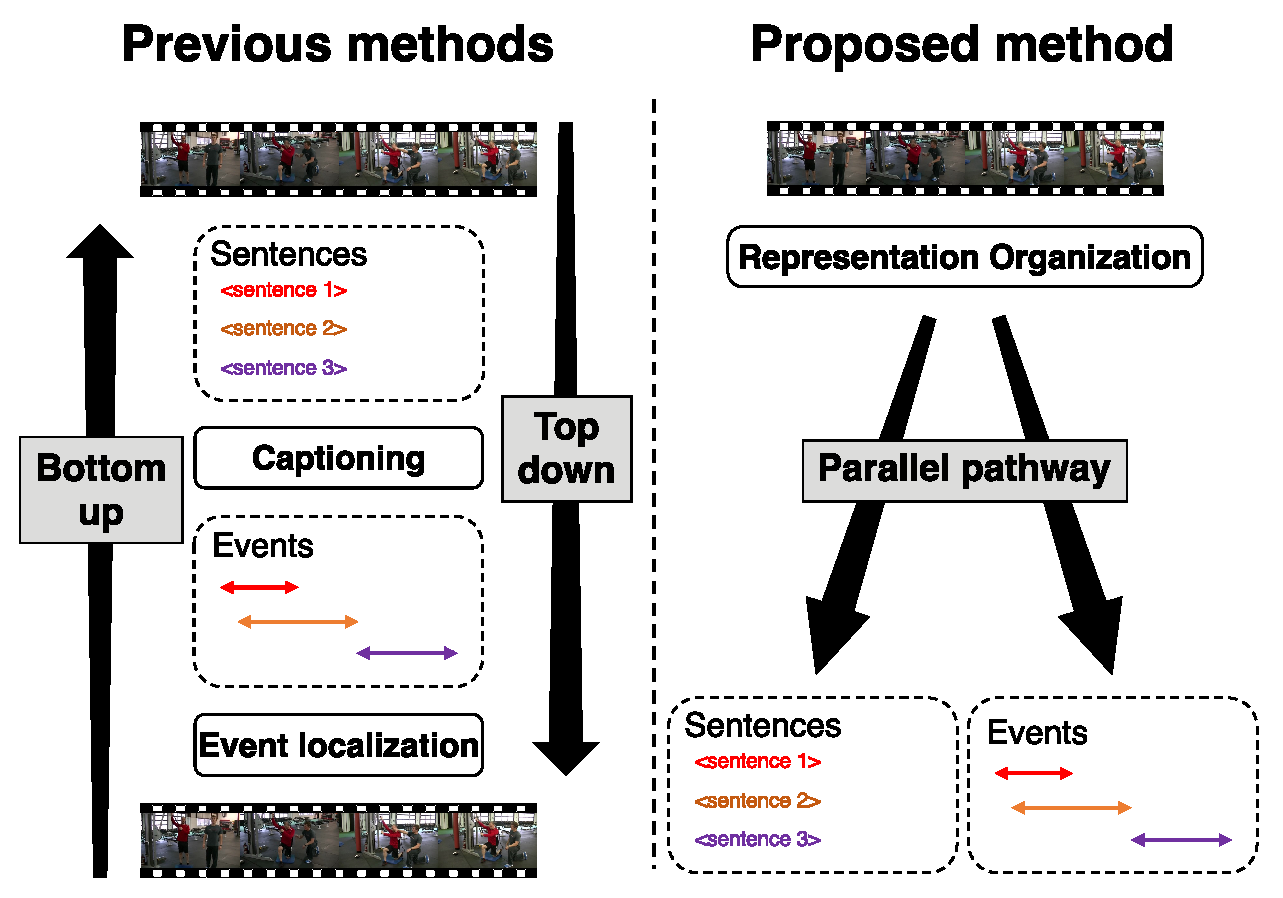
\includegraphics[width=\linewidth]{figures/ppvc_fig1}
  \caption{A summary of comparisons between existing methods and our approach to dense video captioning.}
  \label{fig:intro_approaches}
\end{figure}

\subsection{Limitations of Sequential Processing}

Sequential dense video captioning frameworks can be categorized into two primary paradigms: bottom-up and top-down approaches.
Bottom-up methods~\cite{krishna2017dense,li2018jointly,wang2018bidirectional,zhou2018end,mun2019streamlined} first detect temporal event proposals and subsequently generate corresponding captions, following a ``localize-then-describe'' pipeline.
Conversely, top-down approaches~\cite{deng2021sketch} generate paragraph-level descriptions and then ground individual sentences to specific temporal segments through a ``describe-then-localize'' strategy.

Both paradigms suffer from inherent architectural limitations that constrain their effectiveness.
The most critical issue is \textit{error propagation}: inaccuracies in the initial stage cascade to subsequent modules, creating a compounding effect that degrades overall performance.
In bottom-up approaches, poorly localized events inevitably lead to contextually inappropriate captions, regardless of the sophistication of the language generation module.
Similarly, top-down methods struggle when initial paragraph-level descriptions fail to capture essential temporal structures~\cite{wang2021end}.

Furthermore, sequential approaches typically require \textit{hand-crafted post-processing algorithms} such as Non-Maximum Suppression (NMS) for proposal selection \cite{hosang2017learning}.
These algorithms operate independently of video content, relying solely on temporal overlap criteria and predefined thresholds.
This content-agnostic processing often eliminates semantically meaningful events, particularly in scenarios involving multiple concurrent activities or nested temporal structures.

The sequential dependency also prevents \textit{end-to-end optimization}, necessitating complex multi-stage training procedures that hinder convergence and limit the model's ability to learn optimal joint representations for both localization and captioning tasks~\cite{zhou2018end,wang2021end}.

\subsection{Emergence of Parallel Processing}
Recognizing these fundamental limitations, recent research has explored parallel processing paradigms that perform event localization and caption generation simultaneously~\cite{wang2021end}.
Parallel approaches aim to eliminate sequential dependencies by employing shared encoder representations and parallel decoder heads for the two subtasks.

Wang et al.~\cite{wang2021end} introduced PDVC (Parallel Dense Video Captioning), which demonstrated that parallel decoding could significantly improve performance compared to sequential methods.
However, this pioneering work revealed new challenges specific to parallel architectures: \textit{information bottlenecks at branching points} and \textit{query limitation problems}.

The information bottleneck occurs because parallel approaches still maintain an ``encode-then-decode'' structure, where encoded video features must simultaneously serve both localization and captioning decoders.
This shared representation may not optimally capture the distinct information requirements of each subtask.
Additionally, the limited number of queries in transformer-based decoders restricts the maximum number of detectable events, particularly problematic for long videos containing multiple overlapping activities.

\subsection{Motivation for Enhanced Parallel Architecture}
Our analysis reveals that while parallel processing addresses the error propagation problem inherent in sequential approaches, current implementations fail to fully realize the potential of this paradigm.
The key insight driving our approach is that effective parallel processing requires not merely simultaneous decoding, but architectural innovations that eliminate information bottlenecks while preserving the rich contextual information necessary for both accurate localization and coherent caption generation.

To achieve this goal, we identify three critical design principles:
\begin{enumerate}
  \item Bottleneck-free Information Flow: Instead of forcing all information through a single bottleneck point, we propose passing comprehensive potential information at branching points and filtering unnecessary elements just before decoding. This approach ensures that both localization and captioning modules have access to the full spectrum of relevant visual and temporal information.
  \item Multi-scale Feature Integration: Recognizing that event localization and caption generation may benefit from different levels of feature abstraction, we introduce multi-stack cross-attention mechanisms that enable simultaneous access to both high-level semantic representations and low-level visual details~\cite{vaswani2017attention}.
  \item Dynamic Event Enumeration: Rather than predetermining the number of events through separate counter modules, we propose allowing the model to dynamically determine the optimal number of events based on video content, eliminating artificial constraints on event detection capability.
\end{enumerate}

As illustrated in Figure \ref{fig:intro_approaches}, our proposed Parallel Pathway Dense Video Captioning (PPVC) framework fundamentally reimagines the dense video captioning architecture by eliminating sequential dependencies while addressing the bottleneck limitations of existing parallel approaches.
Through these innovations, PPVC achieves superior performance in both temporal localization accuracy and caption quality compared to state-of-the-art sequential and parallel methods.

The remainder of this chapter details the architectural design and implementation of PPVC, demonstrating how these motivational insights translate into concrete algorithmic improvements that advance the state-of-the-art in dense video captioning.

\section{Parallel Pathway Architecture (PPVC)}
This section describes the core ideas and the network architecture of PPVC in detail.

\subsection{Overview}
For a given video, dense video captioning is the task of detecting multiple overlapping events and generating sentences accordingly.
Existing methods generally divide the whole process into two sub-problems, event detection, and sentence generation, and solve them one by one in order.
The performance of the two modules is tightly coupled, and this sequential processing method causes a major flaw: the result of the preceding module greatly affects the performance of the subsequent module.
However, parallel architectures have the challenge that the bottleneck of information at branch points can limit the outcomes.
Therefore, it is critical to decouple the dependency between the two modules by breaking the sequential processing paradigm while not occurring a bottleneck.

With this consideration, we construct two sub-problems of dense video captioning in parallel.
We first organize the encoded video features into highly relevant ones to understand the core context of the video, rather than directly generating events and sentences from the video.
PPVC consists of five modules: video encoder $\mathcal{E}$, representation organizer $\mathcal{O}$, event localizer $\mathcal{L}$, sentence generator $\mathcal{S}$, gating network $\mathcal{G}$ as depicted in Figure \ref{fig:architecture}. 

Given a video $\mathcal{V}$, it is converted to a hidden state vector $\mathbi{H}_v$ by the video encoder $\mathcal{E}$.
$\mathbi{H}_v$ is fed into the representation organizer $\mathcal{O}$ to organize the encoded video features that determine the context of the video storyline, which is the branch point of the parallel pathway without any bottleneck.
The event localizer $\mathcal{L}$ and sentence generator $\mathcal{S}$ then localize the events $\{e_i\}_{i=1}^{n}$ and generate sentences $\{s_i\}_{i=1}^{n}$, respectively, while further mitigating bottlenecks using multi-stack cross attention.
The gating network $\mathcal{G}$ controls the flow at branch points and refines information by blocking the flow of unnecessary event queries.
The procedure of PPVC is described in Algorithm~\ref{algo:ppvc}.

\begin{sidewaysfigure}
  \centering
   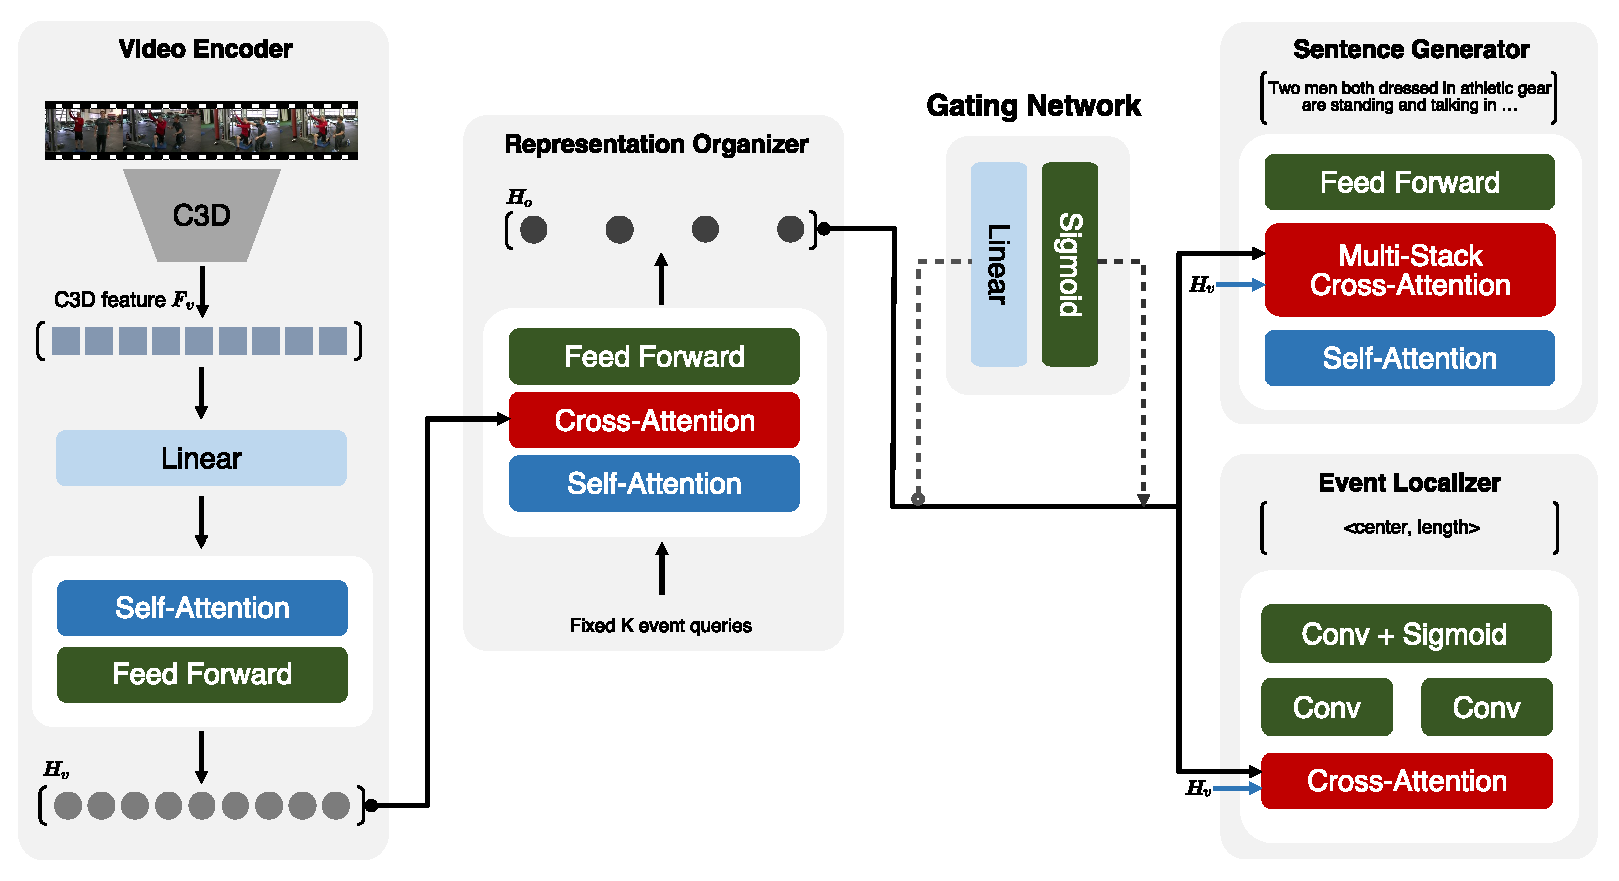
\includegraphics[width=\linewidth]{figures/ppvc_fig2}
   \caption{
    Architecture of the proposed method, PPVC.
   }
  \label{fig:architecture}
\end{sidewaysfigure}

% \begin{figure}[t]
%   \centering
%    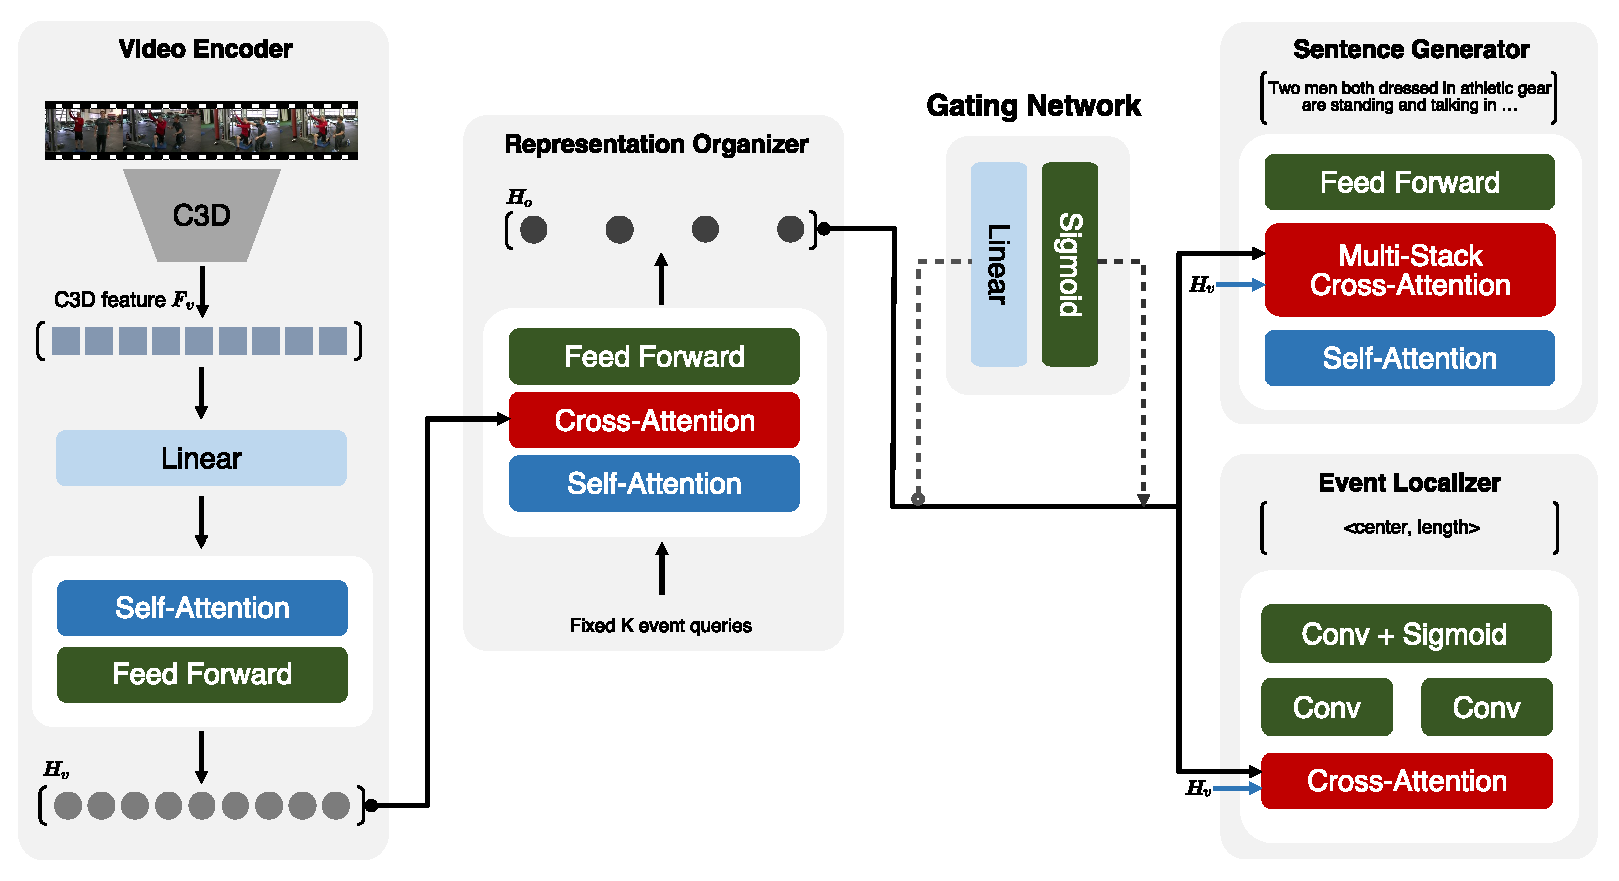
\includegraphics[width=\linewidth]{figures/ppvc_fig2}
%    \caption{
%     Architecture of the proposed method, PPVC.
%    }
%   \label{fig:architecture}
% \end{figure}

\subsection{Video Encoder}
The goal of the video encoder $\mathcal{E}$ is to extract the hidden state $\mathbi{H}_v$ by encoding the spatiotemporal context of the video $\mathcal{V}$.
Our video encoder consists of a convolution network and a sequential data encoder.
In particular, we adopt the C3D~\cite{tran2015learning} network and the transformer encoder~\cite{vaswani2017attention} with multi-head attention (MA) to understand the long-term temporal context of a video.
First, the video encoder divides a given video $\mathcal{V}$ into non-overlapping segments of fixed length (e.g., 8 frames).
The C3D network takes a segment as input and extracts features $\mathbi{F}_v \in \mathbb{R}^{T \times d_f}$, where $T$ is the number of segments and $d_f$ is the dimension of features.
We apply a linear transformation to feed the video feature $\mathbi{F}_v$ of dimension $d_f$ to the transformer encoder~\cite{vaswani2017attention} of dimension $d_m$ as follows:
\begin{equation}
  \mathbi{H}_v^0 = \text{PE} (\text{Linear} \left( \mathbi{F}_v \right) )
  \label{eq:linear_transformation}
\end{equation}
Then, after applying the positional encoding (i.e., $\text{PE}(\cdot)$) to $\text{Linear}(\bm{F}_v)$, we start with the input $\mathbi{H}_v^0$.

\begin{algorithm}[t]
  \caption{Parallel Pathway Dense Video Captioning}
  \label{algo:ppvc}
  \begin{algorithmic}[1]
    \STATE \textbf{Procedure} $\textsc{PPVC}(\mathcal{V})$
    \STATE $\mathbi{H}_v \gets \mathcal{E}(\mathcal{V})$ \COMMENT{Encode video}
    \FOR{$k = 1$ \TO $K$}
      \STATE $\mathbi{H}_o \gets \mathcal{O}(\mathbi{H}_v, \textbf{q}_k)$ \COMMENT{Organize features}
      \STATE $\mathbi{H}_o^{\text{gated}} \gets \mathbi{H}_o \times \mathcal{G}(\mathbi{H}_o)$ \COMMENT{Filter out}
      \STATE \COMMENT{Branch point!}
      \STATE $s_{k} \gets \mathcal{S}(\mathbi{H}_o^{\text{gated}}, \mathbi{H}_v)$ \COMMENT{Describe}
      \STATE $E_{k} \gets \mathcal{L}(\mathbi{H}_o^{\text{gated}}, \mathbi{H}_v)$ \COMMENT{Localize}
    \ENDFOR
    \RETURN $\{E_{k}\}_{k=1}^{K},\;\{s_{k}\}_{k=1}^{K}$
  \end{algorithmic}
\end{algorithm}

The transformer encoder, which contains multiple $N$ layers, is the core of our video encoder.
Each layer is made up of self-attention and feed-forward modules, and at the end of each module, there is a residual connection and layer normalization.
The transformer encoder outputs $\bm{H}_v^{l+1}$  in one cycle given $\mathbi{H}_v^l$, and the output of the last cycle---i.e., the last layer---is $\mathbi{H}_v$.
The following two equations can be used to describe the entire procedure:
\begin{equation}
  \mathbi{H}_v^{l+1} = \text{FFN}\left(\Psi \left(H_v^l + \text{MA}\left( \mathbi{H}_v^l, \mathbi{H}_v^l, \mathbi{H}_v^l \right) \right)\right)
  \label{eq:video_encoder_self_attention}
\end{equation}
\begin{equation}
  \text{FFN}(x) = \text{max} \left(0, x\mathbi{W}_1 + b_1 \right)\mathbi{W}_2 + b_2
  \label{eq:video_encoder_feed_forward}
\end{equation}
\begin{equation}
    \text{MA}(\bm{Q}, \bm{K}, \bm{V}) = \text{Cat}(\{\text{ATT}_i(\bm{Q}, \bm{K}, \bm{V})\}_{i=1}^h)W_O
  \end{equation}
  \begin{equation}
    \text{ATT}(\bm{Q}, \bm{K}, \bm{V}) = \text{softmax}( \frac{(\bm{QW}_Q)(\bm{K}\bm{W}_K)^T}{\sqrt{d_m}} ) (\bm{VW}_V)
  \label{eq:video_encoder_att}
\end{equation}
where, $\Psi\left(\cdot\right)$ represents the layer normalization function.
$\text{Cat}(\cdot)$ denotes vector concatenation and $\bm{W}_*$ are trainable parameters.
We repeat the above process as many times as the number of encoder layers.
Finally, the output of the video encoder is the output of the last layer $\mathbi{H}_v$.

Specifically, the multi-head attention module contains the following two classes of trainable parameters: $\bm{W}_{\{\bm{K},\bm{Q},\bm{V}\}}$ for the query ($\bm{Q}$), key ($\bm{K}$), and value ($\bm{V}$) attention matrix, and $\bm{W}_O$, which is in charge of the output by concatenating attention heads.
The attention head is calculated by scaled dot-product attention, as defined in Equation (\ref{eq:video_encoder_att}), with the same $\bm{H}_v^l$ being served into $\bm{K}$, $\bm{Q}$, and $\bm{V}$ for self-attention.
The final output of multi-head attention is then produced by concatenating all attention heads and applying the weight of $\bm{W}_O$. 
Two linear transformations and a ReLU \cite{agarap2018deep} activation function make up the feed-forward network $\text{FFN}(\cdot)$.
The first linear transformation (i.e., $\bm{W}_1$) and ReLU activation are applied to the output $x$ of multi-head attention. Then it goes through a second linear transformation (i.e., $\bm{W}_2$) with dropout as provided in Equation (\ref{eq:video_encoder_feed_forward}).

The representation organizer inherits the transformer's learning principle.
Specifically, with positional encoding and sequentially input video features, the transformer encoder learns the self-attention between features and organizes features for localization and captioning.
Intuitively, each hidden vector in the outputs of the transformer encoder implicitly contains information for localization and captioning. Therefore, by training in an end-to-end manner from the input to the localization and captioning heads, the representation organizer is trained toward the optimal.

\subsection{Representation Organization}
\label{subsec:method_representation_organization}
Before entering the parallel pathway, we introduce a representation organizer that organizes key encoded video features in the video's spatiotemporal context and uses them as intermediate information for event localization and sentence generation.
The goal of the representation organizer is to extract a representation of salient temporal regions in a video while implicitly producing all potential events.
Specifically, given a video $\mathcal{V}$, representation organizer outputs multiple representations $\mathbi{H}_o$ considering the entire video story.
Later, each representation serves as the core information for an event (i.e., timestamp and sentence), resulting in high-quality event localization and captioning.

For this, we adopt a query-based transformer decoder \cite{carion2020end,zhu2021deformable} because of its high performance and efficiency in object detection tasks using transformers \cite{vaswani2017attention}.
Given the $\mathbi{H}_v$ obtained by the video encoder and the input organized representation vector $\mathbi{H}_o^0$, the representation organizer computes the hidden state $\mathbi{H}_o$ as follows:
\begin{equation}
  \mathbi{H}_o^{\text{self}} = \Psi \left( \mathbi{H}_w^l + \text{MA} \left(\mathbi{H}_o^l, \mathbi{H}_o^l, \mathbi{H}_o^l \right) \right)
  \label{eq:representation_organization_self_attention}
\end{equation}
\begin{equation}
  \mathbi{H}_o^{\text{cross}} = \Psi \left( \mathbi{H}_o^{\text{self}} + \text{MA} \left( \mathbi{H}_o^{\text{self}}, \mathbi{H}_v, \mathbi{H}_v \right) \right)
  \label{eq:representation_organization_cross_attention}
\end{equation}
\begin{equation}
  \mathbi{H}_o^{l+1} = \Psi \left( \mathbi{H}_o^{\text{cross}} + \text{FFN}\left( \mathbi{H}_o^{\text{cross}} \right) \right)
  \label{eq:representation_organization_ffn}
\end{equation}
where, MA($\cdot$), FFN($\cdot$) and $\Psi \left(\cdot\right)$ are the same as used in Equation \ref{eq:video_encoder_self_attention} and Equation \ref{eq:video_encoder_feed_forward}.
$l$ is the sequence number of the transformer decoder.
The output of the last layer is $\mathbi{H}_o \in \mathbb{R}^{K \times d_m}$ ($K$ is the number of generated representations).

Here, as described above, we set the number of event queries to a fixed number of $K$ without depending on the event counter.
The event counter is likely to output the average number regardless of the content based on the statistics of the entire dataset.
We control the number of events by generating events for fixed $K$ event queries (i.e., the maximum number of events that PPVC can generate.) and removing unnecessary ones.

\textbf{Choice of $K$.}
Determining $K$ requires great care as it limits the maximum number of events that PPVC can generate.
With a high $K$, PPVC generates many events, so recall can be high, but precision is not guaranteed. 
On the other hand, a low $K$ increases precision, but does not guarantee high recall in videos containing many events.
Therefore, we empirically set $K$ to 10 to measure the F1 score by varying $K$ to strike the balance between recall and precision (details in Section \ref{subsec:experiments-ablation_study}).

\subsection{Event Localizer}
\label{subsec:method_event_localizer}
The goal of the event localizer is to predict the center and duration of an event in the video corresponding to an organized representation.
Common problems with the event localizer are that it is difficult to predict how many events are included in the video, and the events must be determined by considering the correlations between events.
Our event localization approach implicitly determines the number of events (i.e., the number of organized representations) in the previous step (representation organization), without an event counter or a proposal generation network.
Therefore, this section only focuses on the localization of the timestamps corresponding to the organized representations in the entire video.

The event localizer is based on the transformer decoder \cite{vaswani2017attention}.
The difference from the basic transformer decoder is that it does not have a self-attention block (i.e., not auto-regressive) and directly regresses the timestamp through several convolutional neural networks after the cross-attention block.
For each organized representation $\mathbi{H}_o$, we use a multi-head attention module to incorporate the entire video storyline (i.e., encoded video feature $\mathbi{H}_v$) as follows:
\begin{equation}
  \mathbi{H}_e^{\text{cross}} = \Psi \left( \mathbi{H}_e^{\text{self}} + \text{MA} \left( \mathbi{H}_e^{\text{self}}, \mathbi{H}_{v}, \mathbi{H}_{v} \right) \right)
  \label{eq:event_localizer_cross_attention}
\end{equation}
We then apply several 1D convolutional layers on the temporal dimension and predict the ratio of center and duration timestamps to the entire video using two linear regression heads.

\subsection{Sentence Generator}
\label{subsec:method-sentence_generator}
The goal of the sentence generator $\mathcal{S}$, the second part of the parallel pathway, is to receive organized representations $\{\mathbi{H}_o^i\}_{i=0}^{N}$ from the representation organizer and generate sentences ${\{s_i\}}_{i=0}^{N}$: $\mathcal{S}\left({\{\mathbi{H}_o^i\}_{i=0}^{N}}\right) \rightarrow {\{s_i\}}_{i=0}^{N}$.
One of the important points in sentence generation in a dense video captioning task is to maintain coherency.
There are several approaches to this, but we guarantee coherency between sentences by directly incorporating the textual features of the video.
Directly merging video features instead of merging past sentences improves sentence coherency while avoiding referencing ill-defined words in the last sentence.

Our sentence generator is based on a transformer decoder \cite{vaswani2017attention}, and most of the process is similar to $\mathcal{O}$.
The difference from the basic transformer decoder is that there are two hidden states (i.e., two pairs of key and value) that are input to the cross-attention block: the visual hidden state $\mathbi{H}_v$ and the organized representation $\mathbi{H}_o$.
Therefore, we design a multi-stack cross-attention module that refers to multiple hidden states.
This applies the multi-head attention module sequentially to two or more hidden states by stacking, which makes it possible to utilize various information during decoding.

The sentence generation process using multi-stack cross-attention is as follows:
\begin{equation}
  \mathbi{H}_s^{\text{cross}^1} = \Psi \left( \mathbi{H}_s^{\text{self}} + \text{MA} \left( \mathbi{H}_s^{\text{self}}, \mathbi{H}_{v}, \mathbi{H}_{v} \right) \right)
  \label{eq:setence_constructor_cross1_attention}
\end{equation}
\begin{equation}
  \mathbi{H}_s^{\text{cross}^2} = \Psi \left( \mathbi{H}_s^{\text{cross}^1} + \text{MA} \left( \mathbi{H}_s^{\text{cross}^1}, \mathbi{H}_{w}, \mathbi{H}_{w} \right) \right)
  \label{eq:setence_constructor_cross2_attention}
\end{equation}
Note that we omit positional encoding, self-attention, and feed-forward processes because they are the same as the representation organizer (Section \ref{subsec:method_representation_organization}).

\subsection{Gating Network}
\label{subsec:method-gating_network}
In addition to the modules described above, we employ a gating network that signals the end of a sequence of the representation organizer and controls the flow into parallel pathways.
Since the representation organizer creates all of the possible organized representations, it is necessary to prevent the generation of redundant or unnecessary events by indicating the end of the sequence and limiting the flow of parallel pathways.
In other words, the gating network consequently serves to increase precision in event localization.
Our gating network outputs a confidence score for the organized representation through the sigmoid activation function after linear transformation as follows:
\begin{equation}
  g(x) = \sigma (\text{Linear}(x))
\end{equation}
\begin{equation}
  \mathbi{H}_o^{\text{gated}} = g(\mathbi{H}_o) \cdot \mathbi{H}_o
  \label{eq:gating_network}
\end{equation}
It is simple but effective, prevents unnecessary representation generation, and as a result helps high-quality localization and captioning.

\section{Experimental Evaluation}
\subsection{Dataset}
\label{subsec:experiments-dataset}

% \begin{table*}[t]
\begin{sidewaystable}
  \centering
  \caption{
    Performance comparison of the event localization.
  }
  \begin{tabular}{@{}l|c|ccccc|ccccc|c@{}}
    \hline
    % Method & Recall (@tIoU) & Precision (@tIoU) \\
    % & \multicolumn{5}{l}{} & \multicolumn{5}{l}{} \\
    \multirow{2}{*}{Method} & \multirow{2}{*}{PN} & \multicolumn{5}{|c|}{Recall (@tIoU)} & \multicolumn{5}{c}{Precision (@tIoU)} & \multirow{2}{*}{F1} \\
    && @0.3 & @0.5 & @0.7 & @0.9 & Average & @0.3 & @0.5 & @0.7 & @0.9 & Average & \\
    \hline
    MFT'18 \cite{xiong2018move} & $\checkmark$ & 46.18 & 29.76 & 15.54 & 5.77 & 24.31 & 86.34 & 68.79 & 38.30 & 12.19 & 51.41 & 33.01 \\
    SDVC'19 \cite{mun2019streamlined} & $\checkmark$ & 93.41 & 76.40 & 42.40 & 10.10 & 55.58 & 96.71 & 77.73 & 44.84 & 10.99 & 57.57 & 56.56 \\
    PDVC'21 \cite{wang2021end} &  & 89.47 & 81.91 & 44.63 & 15.67 & 55.42 & 97.16 & 78.09 & 42.68 & 14.40 & 58.07 & 56.71 \\
    \textbf{PPVC} &  & 91.71 & 78.90 & \textbf{56.73} & \textbf{20.60} & \textbf{61.98} & 96.23 & 73.80 & 37.66 & 12.61 & 55.07 & \textbf{58.33} \\
    \hline
  \end{tabular}
  
  \label{tab:eval_event_localizer}
% \end{table*}
\end{sidewaystable}

% \begin{table*}[tp]
\begin{sidewaystable}
  \centering
  \caption{
    Performance comparison of the dense video captioning (ActivityNet Captions validation set).
  }
  \begin{tabular}{@{}l|ccc|cc|ccccccc@{}}
    \hline
    % Method & Recall (@tIoU) & Precision (@tIoU) \\
    % & \multicolumn{5}{l}{} & \multicolumn{5}{l}{} \\
    % \multirow{2}{*}{Method} & \multicolumn{6}{|c|}{with GT events} & \multicolumn{6}{c}{with predicted events} \\
    \multirow{2}{*}{Method} & \multicolumn{3}{|c|}{Feature} & \multicolumn{2}{|c|}{Training} \\
     & C3D & TSN & Optical & CE & RL & B@1 & B@2 & B@3 & B@4 & C & M\\
     \hline
    DCE'17 \cite{krishna2017dense}        & $\checkmark$ & & & $\checkmark$ & & 10.81 & 4.57  & 1.90  & 0.71 & 12.43 & 5.69\\
    TDA-CG'18 \cite{wang2018bidirectional} & $\checkmark$ & & & $\checkmark$ & & -     & -     & -     & 1.31  & 7.99 & 5.86\\
    DVC'18 \cite{li2018jointly}            & $\checkmark$ & & & $\checkmark$ & & 12.22 & 5.72  & 2.27  & 0.73 & 12.61 & 6.93\\
    Efficient'20 \cite{suin2020efficient}  & $\checkmark$ & & & $\checkmark$ & & -     & -     & 2.87  & 1.35 & 13.82 & 6.21\\
    ECHR'20 \cite{wang2020event}           & $\checkmark$ & & & $\checkmark$ & & -     & -     & -     & 1.29 & 14.71 & 7.19\\
    WS-DEC'21 \cite{chen2021towards}*      & $\checkmark$ & & & $\checkmark$ & & 13.36 & 5.96  & 2.78  & 1.33 & 21.21 & 7.49\\
    PDVC'21 \cite{wang2021end}             & $\checkmark$ & & & $\checkmark$ & & -     & -     & -     & 1.65 & 25.87 & 7.50 \\
    \textbf{PPVC}                       & $\checkmark$ & & & $\checkmark$ & & \textbf{14.93} & \textbf{7.40}  & \textbf{3.58}  & \textbf{1.68} & 23.02 & \textbf{7.91} \\
    \hline
    MT'18 \cite{zhou2018end} & & $\checkmark$ & $\checkmark$ & $\checkmark$   & & 9.96 & 4.81 & 2.42 & 1.15 & 9.25 & 4.98 \\
    SDVC'19 \cite{mun2019streamlined} & $\checkmark$ & & & $\checkmark$ & $\checkmark$ & 17.92 & 7.99 & 2.94 & 0.93 & 30.68 & 8.82 \\
    SGR'21 \cite{deng2021sketch} & $\checkmark$ & & & $\checkmark$ & $\checkmark$ & 14.05 & - & - & 1.67 & 22.12 & 9.07 \\
    \hline
  \end{tabular}
  \label{tab:eval_captioner}
% \end{table*}
\end{sidewaystable}

\begin{table}[tp]
  \centering
  \caption{
    Performance comparison of the dense video captioning (YouCook2-TSN).
  }
  \begin{tabular}{@{}l|c|c|cccc|ccccc|c@{}}
    \hline
    Method &  B@4 & C &  M \\
    \hline
    MT'18 \cite{zhou2018end} & 0.30 &  6.10 &  3.18 \\
    ECHR'18 \cite{wang2018bidirectional} & - & - &  3.82 \\
    PDVC'21 \cite{wang2021end} &  0.80 &  22.71 &  4.74 \\
    SGR'21 \cite{deng2021sketch} & - &  - &  4.35 \\
    \textbf{PPVC} &  \textbf{0.89} &  19.70 &  \textbf{4.94} \\
    \hline
  \end{tabular}
  \label{tab:eval_captioner_yc2}
\end{table}

We evaluate the performance of our framework on the two large-scale benchmark datasets, ActivityNet Captions \cite{krishna2017dense} and YouCook2 \cite{zhou2018towards}.
The ActivityNet Captions dataset contains 19,994 Youtube videos, which are divided into three subsets: 10,009, 4,917, and 4,885 videos for training, validation, and testing, respectively.
% We evaluate the performance of our framework on the ActivityNet Captions dataset \cite{krishna2017dense}, which contains 19,994 Youtube videos.
% They are divided into three subsets with 10,009, 4,917 and 4,885 videos for training, validation, and testing, respectively.
On average, the length of videos is 120 seconds, and each video has 3.65 pairs of events and sentences.
Each sentence has, on average, 13.48 words.
YouCook2 has 2,000 untrimmed videos of cooking activities with an average length of 320 seconds.
The videos have 7.7 events and sentences on average.
We use C3D \cite{tran2015learning} and TSN \cite{wang2018temporal} features for fair comparison for the ActivityNet Captions dataset and the YouCook2 dataset, respectively.
C3D features are obtained by passing non-overlapping, fixed-length video segments of 8 frames to the C3D network pre-trained on Sports-1M \cite{karpathy2014large}.

\subsection{Metrics}
\label{subsec:experiments-metrics}

We use publicly available evaluation code\footnote{\url{https://github.com/ranjaykrishna/densevid_eval}} provided by the ActivityNet Captions Challenge.
We measure recall and precision of event localization and METEOR \cite{banerjee2005meteor}, CIDEr \cite{vedantam2015cider} and BLEU \cite{papineni2002bleu} of sentences.
Given a generated event and sentence pair, if its event has an overlapping larger than the threshold with any ground-truth events, the captioning score is computed by comparing the corresponding ground-truth sentence.
Otherwise, the score is set to 0.


% METEOR is a widely used metric of the ActivityNet Captions challenge, but it tends to score high for redundant captions that are difficult for humans to read.
% METEOR inherently has a gap between what human prefer to read and what machines can generate.
% To circumvent such pitfall, we use SODA(c) \cite{fujita2020soda} as an evaluation metric, which is a story-oriented dense video captioning evaluation framework.
% SODA(c) is based on METEOR, however it penalizes duplicated captions.
% Thus, higher scores are given for captions that are equal to the number reference captions.
% We include SODA(c) because it reflects human readability better than METEOR.


\subsection{Implementation Details}
\label{subsec:experiments-impl_details}

For all modules, the hidden size $d_m$ of multi-head attention is 512, the number of attention heads is 8, and the encoder and decoder have 6 layers.
The feed-forward network used in the encoder and decoder is 2,048 dimensions.
The residual and attention dropout ratio is 0.1.
To prevent over-fitting, we apply dropout to the visual input embedding layer.
We train the model with adamW \cite{loshchilov2017decoupled} for 30 epochs with a batch size of 1.
We vary the learning rate as in \cite{vaswani2017attention} and set warmup steps to 10 epochs, which initially increases linearly from 0 to about 0.00005, and then decreases proportionally to the inverse square root.
The label smoothing factor is set to 0.1.

\subsection{Performance Comparison}
\label{subsec:experiments-perfom_comp}
We compare the performance of PPVC with several state-of-the-art methods \cite{krishna2017dense,wang2018bidirectional,li2018jointly,zhou2018end,mun2019streamlined,suin2020efficient,wang2020event,chen2021towards,deng2021sketch,wang2021end}.



\textbf{Event localization.}
We first compare the performance of the event localizer among the two subtasks and present the results in Table \ref{tab:eval_event_localizer}.
We evaluate the localization performance of PPVC with respect to the 4 temporal intersections of unions (@tIoU) thresholds on the Activity Captions validation set.
PN stands for proposal network.


MFT, SDVC, and PDVC explicitly detect events through the event proposal networks.
In contrast, our method uses the representation organizer to roughly compose representations of the events (i.e., implicit) and then localize each representation.
Our event localizer achieves superior performance over MFT, SDVC, and PDVC in terms of F1 score.
Specifically, PPVC surpasses MFT by a large margin, and although its precision is slightly lower than SDVC and PDVC, its recall is slightly superior, resulting in a higher F1 score.
Based on these results, we can confirm the effectiveness of the representation organizer, the event localizer, and the gating network without any proposal network.

\textbf{Dense video captioning.}
Tables \ref{tab:eval_captioner} and \ref{tab:eval_captioner_yc2} show the comparisons of captioning performance for state-of-the-art methods using BLEU@N (B@N), CIDEr (C) and METEOR (M) on the ActivityNet validation set and YouCook2 dataset, respectively.
Asterisk (*) indicates methods evaluated under an incomplete dataset (e.g., 80\%) due to a download issue.
CE and RL stand for cross-entropy and reinforcement learning, respectively.
PPVC achieves superior performance compared to the state-of-the-art scheme in terms of the widely used METEOR metric in the ActivityNet Captions challenge.

A few methods \cite{mun2019streamlined,deng2021sketch,wang2020event} adopt reinforcement learning to further improve performance after cross-entropy training.
They require extra-long training time for RL training and most importantly they tend to generate repetitive phrases \cite{wang2019describing}.
The RL fine-tuning approach expects high metric values but yields rather poor results in terms of human readability.
In short, metrics such as CIDEr and METEOR cannot perfectly evaluate human readability.
In this paper, since we attach great importance to both quantitative and qualitative results, we do not adopt the RL training in the language model.

\begin{table}[t]
  \centering
  \caption{
    A performance comparison of the dense video captioning with ground-truth proposals.
    % A summary of the performance comparison using BLEU@4 (B@4), CIDEr (C), and METEOR (M) with ground-truth proposals on the ActivityNet validation set.
  }
  \begin{tabular}{l|c|c|c}
    \hline
    Method & B@4 & C & M \\
    \hline
    DCE'17 \cite{krishna2017dense} & 1.60 & 8.88 & 25.12 \\
    TDA-CG'18 \cite{wang2018bidirectional} & - & 9.69 & - \\
    DVC'18 \cite{li2018jointly} & 1.62 & 10.33 & 25.24 \\
    ECHR'20 \cite{wang2020event} & 1.96 & 10.58 & 39.73 \\
    PDVC'21 \cite{wang2021end} & 2.64 & 10.54 & 47.26 \\
    \textbf{PPVC} & \textbf{2.76} & 10.48 & \textbf{49.31} \\
    \hline
  \end{tabular}
  \label{tab:eval_captioning_gt}
\end{table}

Note that, we exclude comparison methods that use anything other than C3D/TSN features (i.e., multi-modal) or train the captioning module with reinforcement learning after cross-entropy training.
RL adopts a natural language evaluation metric such as METEOR directly as a reward, which is very effective for high scores. 
However, it tends to generate repetitive phrases with long sentences \cite{wang2019describing}, which reduces readability \cite{wang2018bidirectional,fujita2020soda}.
In this work, we do not use the RL training in the language model since we place a high value on both quantitative and qualitative results.

We evaluate the PPVC with ground-truth proposals, examining only the captioning performance separately from event localization on the ActivityNet validation set, as shown in Table \ref{tab:eval_captioning_gt}.
Compared to other algorithms, PPVC is slightly inferior in CIDEr but superior in BLEU@4 and METEOR metrics, indicating that the events generated by PPVC are more accurate.
We also compare the performance of PPVC with the state-of-the-art methods on the YouCook2 dataset, as shown in Table \ref{tab:eval_captioner_yc2}.
Similarly, PPVC outperforms other algorithms in terms of METEOR and BLEU@4.
Based on these results, we can see that PPVC is effective with parallel pathways instead of sequential paradigms.
Compared to PDVC, which is a similar parallel decoding approach, PPVC achieves slightly better results in terms of BLEU and METEOR, indicating the effectiveness of representation organizers over event counter head.

We analyze PPVC in depth based on the evaluation mechanisms and values of the metrics.
CIDEr (Consensus-based Image Description Evaluation) is a TF-IDF (Term Frequency-Inverse Document Frequency)-based natural language evaluation metric.
By taking into account both the frequency of the words and the length of the document, TF-IDF determines the importance of each word.
CIDEr evaluates a candidate sentence by vectorizing the TF-IDF values of words in the candidate sentence and reference sentences and comparing their similarity.
Intuitively, it tends to ignore grammar and word order and concentrate more on event-specific words than common words in reference sentences.
METEOR (Metric for Evaluation of Translation with Explicit ORdering), on the other hand, evaluates a candidate sentence using a penalty function for inconsistencies and weighted F-score (i.e., both recall and precision).
It takes into account the portion of the generated sentence where the n-grams match those of the reference sentences.
We contend, based on these facts, that PPVC has advantages in terms of sentence completeness using common words and drawbacks in generating event-specific words.

\begin{table}[t]
  \centering
  \caption{
    Average number of events per video.
    % Average number of events per video generated by the event localizer on ActivityNet Caption validation set.
    % PN, NMS and EC are proposal network, non-maximum suppression and event counter, respectively.
  }
  \begin{tabular}{l|c|c}
    \hline
    Method & Approach & Num. events \\
    \hline
    SDVC'19 \cite{mun2019streamlined} & PN+NMS & 2.85 \\
    PDVC'21 \cite{wang2021end} & EC & 3.03\\
    \textbf{PPVC} & - & 5.54 \\
    % Avg. number of GT events & & 3.65 \\
    \hline
  \end{tabular}
  \label{tab:eval_num_events}
\end{table}

\begin{figure}[t]
  \centering
%   \includegraphics[width=0.9\linewidth]{figures/distribution_num_events}
   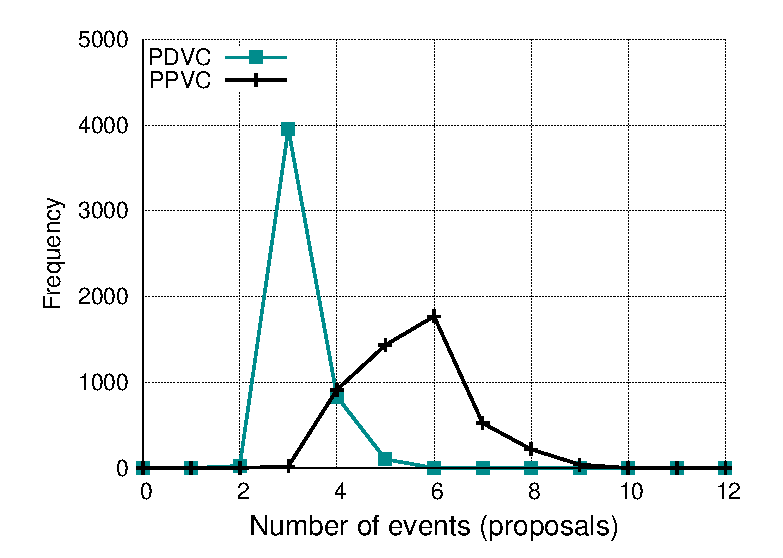
\includegraphics[width=0.9\linewidth]{figures/ppvc_fig3}
   \caption{
    Distribution of the number of events per video.
    % Distribution of the number of events generated by PDVC and PPVC.
    % PPVC generates more events and sentences on average, indicating a richer description of the video.
   }
   \label{fig:eval_dist_events}
\end{figure}

\textbf{Representation organization.}
For a more in-depth analysis of representation organizers, we examine the events generated from all videos included in the ActivityNet Captions validation set.
Table \ref{tab:eval_num_events} and Figure \ref{fig:eval_dist_events} show the number of events generated from each method, and the distribution of the number of events generated for all videos, respectively.
In Table {\ref{tab:eval_num_events}}, PN, NMS, and EC are proposal network, non-maximum suppression, and event counter, respectively.

In PPVC, the number of events is widely distributed from 3 to 9, whereas PDVC generates only 3 to 5 events per video.
In terms of the average number, PPVC, PDVC, and SDVC generate 5.54, 3.03, and 2.85 events, respectively, indicating that PPVC generates more sentences and a more detailed description of the video.

Furthermore, based on the above results, the event counter of PDVC outputs 3 (80.4 \%), which is the average of the number of events of the videos in the entire dataset.
On the other hand, PPVC without an event counter generates proposals with a more diverse number of events.





\begin{figure}[t]
  \centering
%   \includegraphics[width=0.9\linewidth]{figures/eval_ablation}
   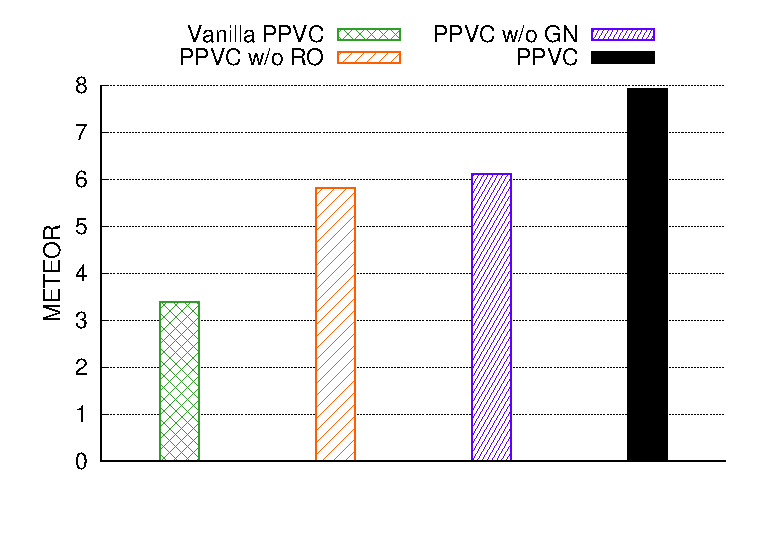
\includegraphics[width=0.9\linewidth]{figures/ppvc_fig4}
   \caption{
    The ablation result of each module for captioning.
    % Ablation results on ActivityNet Captions validation set.
    % Vanilla PPVC means a simple parallel pathway model without both the representation organizer and the gating network used in the full model.
    % ``RO" and ``GN" stand for the representation organizer and the gating network, respectively.
    }
   \label{fig:eval_ablation}
   \end{figure}

\begin{table}[t]
   \centering
   \caption{
      The ablation result of each module for localization.
    %   Ablation results of average recall and precision on the ActivityNet Captions validation set.
    %   Vanilla PPVC means a simple parallel pathway model without the representation organizer and the gating network used in the full model.
    % ``RO" and ``GN" stand for the representation organizer and the gating network, respectively.
   }
   \begin{tabular}{l|c|c}
      \hline
      Method & Recall & Precision \\
      \hline
      Vanilla    & 44.53 & 32.92 \\
      W/o RO    & 77.90 & 34.57 \\
      W/o GN    & 74.37 & 39.93 \\
      Full       & 61.98 & 58.33 \\
      \hline
  \end{tabular}
  \label{tab:eval_ablation_event_localization}
 \end{table}
 


\subsection{Ablation Study}
\label{subsec:experiments-ablation_study}
\textbf{Ablation study on each module.}
We conduct several ablation studies to precisely quantify the contribution of the core modules of PPVC.
We compare the performance of 4 different models with different combinations of modules as follows: (i) vanilla PPVC: has a parallel pathway but no representation organizer and gating network, (ii) PPVC without representation organizer: directly localizes and describes the events from the encoded video, (iii) PPVC without gating network: does not control the flow to the event localizer and the sentence generator, (iv) PPVC (full model).

Figure {\ref{fig:eval_ablation}} and Table {\ref{tab:eval_ablation_event_localization}} show the average recall and precision (i.e., localization) of an ablation study on the ActivityNet validation set and we have the following observations.
``RO" and ``GN" stand for the representation organizer and the gating network, respectively.
First, vanilla PPVC eliminates the dependency between the two modules with a parallel architecture, however, suffers from localizing and describing events directly from the vast amounts of video features.
We argue that the simple parallel pathway dense video captioning model may not be as effective as the conventional sequential method.
Second, applying the representation organizer to vanilla PPVC, it can be seen that there is a significant performance gain.
This result proves that the representation organizer acts as a filter to extract only the necessary (core) information and guides the event localizer and sentence generator.
Third, the gating network is essential in PPVC because it controls the flow from the representation organizer to the parallel pathway and filters the unnecessary representations.
%

\begin{figure}[t]
  \centering
%   \includegraphics[width=0.9\linewidth]{figures/eval_ablation_num_query.eps}
   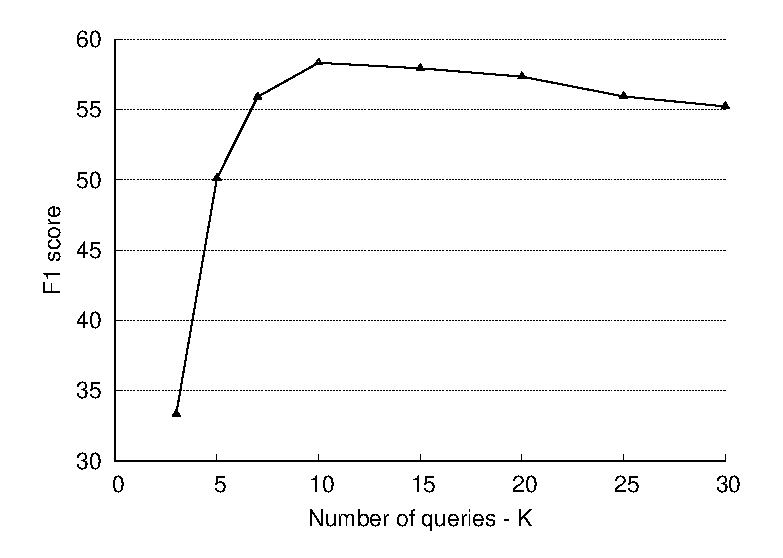
\includegraphics[width=0.9\linewidth]{figures/ppvc_fig5}
   \caption{
    The ablation result of the number of queries.
    % Ablation results on ActivityNet Captions validation set.
    % We measure the F1 score by varying $K$, the number of fixed queries in PPVC.
   }
   \label{fig:eval_ablation_num_query}
\end{figure}



\textbf{Ablation study on the number of queries.}
We train several times to determine the number of fixed queries, $K$, and measure F1 for the generated events by varying $K$.
Based on the fact that the ActivityNet Captions dataset contains videos of up to 27 events, we examine the results for $K$ of 3, 5, 7, 10, 15, 20, 25, and 30.
It can be seen that the best performance is when the number of queries is 10, as shown in Figure \ref{fig:eval_ablation_num_query}.
The overall performance tends to improve as the number of queries rises, but when it exceeds 10, it starts to somewhat decline.
PPVC has the following trade-offs, depending on the number of queries: Low query numbers cause PPVC to have a low recall in event localization; on the other hand, high query numbers cause a high recall but poor precision.
Consequently, we set $K$ to 10 for the number of queries, which is the best F1 score (i.e., the harmonic mean of the recall and precision).

In short, by eliminating bottlenecks caused by the representation organizer and the gating network, PPVC achieves performance improvements over PDVC, an existing parallel decoding method.
Figure \ref{fig:eval_ablation} demonstrates the efficiency of the representation organizer and the gating network, while Figure \ref{fig:eval_ablation_num_query} demonstrates the need for a larger number of queries.

\begin{sidewaysfigure}
\centering
  % \fbox{\rule{0pt}{5in} \rule{1\linewidth}{0pt}}
%  \includegraphics[width=1\linewidth]{figures/eval_qualitative}
  \includegraphics[width=0.8\columnwidth]{figures/ppvc_fig6}
  \caption{
    Examples of qualitative results on ActivityNet Captions validation set.
    Sentences corresponding to the event are matched with the same color.
  }
  \label{fig:eval_qualitative_results}
\end{sidewaysfigure}

% \begin{figure*}[!tp]
%   \centering
%   % \fbox{\rule{0pt}{5in} \rule{1\linewidth}{0pt}}
% %  \includegraphics[width=1\linewidth]{figures/eval_qualitative}
%   \includegraphics[width=1\linewidth]{figures/ppvc_fig6}
%   \caption{
%     Examples of qualitative results on ActivityNet Captions validation set.
%     Sentences corresponding to the event are matched with the same color.
%   }
%   \label{fig:eval_qualitative_results}
% \end{figure*}

\subsection{Qualitative Results}
\label{subsec:experiments-qual_res}

Figure \ref{fig:eval_qualitative_results} illustrates the qualitative results of localizing and describing events in the video.
First, it can be seen that PPVC localizes and describes videos with a large number of events (i.e., more than 4) in both examples.
To detect more events, PPVC has two mechanisms: the representation organizer (Section \ref{subsec:method_representation_organization}) and the gating network (Section \ref{subsec:method-gating_network}).
The representation organizer implicitly generates all possible events based on the number of queries.
Then, the gating network eliminates unnecessary events to determine the final events of PPVC.

Second, We can see that PPVC generates fluent and rich sentences using the keywords such as ``kayak'', ``waves'', ``bumpy'', ``dog'', ``man'', ``frisbee'' and ``catch'' in both examples.
Unfortunately, there are some ill-defined sentences in the black and pink sentences in the second video.
PPVC generates the same sentence for two different events.
However, generating repeated sequences is one of the common challenges of language models.
We leave reducing this by contributing to sentence generation as our future work.

\section{Advantages and Limitations}
\label{sec:advantages_limitations}

The Parallel Pathway Dense Video Captioning (PPVC) framework introduces significant architectural innovations that address fundamental limitations of sequential processing paradigms while introducing new challenges inherent to parallel transformer-based architectures. This section provides a comprehensive analysis of the advantages and limitations of our proposed approach.

\subsection{Advantages}

\textbf{Elimination of Error Propagation.}
The most significant advantage of PPVC lies in its ability to eliminate the error propagation problem that plagues sequential dense video captioning methods~\cite{Krishna2017-pw,Li2018-ll,Wang2018-ap}.
By performing event localization and caption generation simultaneously rather than sequentially, PPVC prevents localization errors from cascading to the captioning module.
This architectural design ensures that both subtasks have access to the same rich visual representations, enabling more robust and accurate dense video captioning performance as demonstrated in our experimental results.

\textbf{Bottleneck-Free Information Flow.}
Traditional parallel approaches suffer from information bottlenecks at branching points where encoded features must serve both localization and captioning decoders~\cite{Wang2021-zi}. PPVC addresses this limitation through its representation organizer module, which extracts comprehensive potential information before branching and filters unnecessary elements just before decoding. This design ensures that both pathways receive rich, contextually relevant features without artificial constraints imposed by limited intermediate representations.

\textbf{Enhanced Feature Utilization through Multi-Stack Cross-Attention.}
The multi-stack cross-attention mechanism represents a key innovation that enables simultaneous access to both organized high-level features and raw low-level visual information~\cite{Vaswani2017-sc}. This dual-pathway feature utilization addresses the limitation that individual attention heads may focus on different aspects of the input, allowing the model to leverage complementary information sources for improved localization and captioning accuracy. The parallel processing of multi-head attention mechanisms provides computational efficiency while maintaining the model's ability to capture complex temporal relationships~\cite{Dosovitskiy2021-vn}.

\textbf{Content-Aware Event Detection.}
Unlike conventional approaches that rely on hand-crafted algorithms such as Non-Maximum Suppression (NMS)~\cite{hosang2017learning}, PPVC employs a gating network that makes content-aware decisions about event relevance. This eliminates the risk of removing semantically important but temporally overlapping events, which is particularly crucial for complex video scenarios where multiple concurrent activities occur. Our results demonstrate that PPVC generates significantly more events per video (5.54 vs. 3.03 for PDVC), enabling richer and more detailed video descriptions.

\textbf{End-to-End Optimization.}
The parallel architecture enables true end-to-end optimization without the complex multi-stage training procedures required by sequential methods~\cite{Zhou2018-zu}. This unified training approach allows the model to learn optimal joint representations for both localization and captioning tasks, leading to improved overall performance and training stability.

\subsection{Limitations}
\textbf{Fixed Query Limitations and Scalability Constraints.}
A fundamental limitation of PPVC lies in its reliance on a fixed number of queries ($K=10$) to determine the maximum number of detectable events.
This design choice creates an inherent trade-off between recall and precision: low query numbers limit recall for videos with many events, while high query numbers may decrease precision due to false positive generation. Although our empirical analysis determined the optimal value through F1 score optimization, this constraint may limit the framework's applicability to videos with highly variable event densities or exceptionally complex temporal structures.

\textbf{Computational Complexity and Memory Requirements.}
The transformer-based architecture, while enabling parallel processing, introduces significant computational overhead due to the quadratic complexity of self-attention mechanisms~\cite{Vaswani2017-sc}. Specifically, the computational complexity scales as $O(n^2 \cdot d + n \cdot d^2)$, where n represents the sequence length and d denotes the feature dimension.
This quadratic scaling in both time and memory requirements can become prohibitive for long video sequences, particularly when processing untrimmed videos that may contain hundreds or thousands of temporal segments. Recent work has established theoretical lower bounds proving that self-attention complexity is necessarily quadratic unless strong computational assumptions are violated~\cite{duman2023computational}.

\textbf{Residual Sequential Characteristics.}
Despite the parallel decoding architecture, PPVC maintains an encoding-then-decoding structure that preserves some sequential characteristics. The video encoder processes the entire input sequence before parallel pathways begin operation, potentially creating a bottleneck where poorly encoded features can negatively impact both localization and captioning performance. This limitation suggests that future architectures might benefit from more thoroughly parallel processing that extends to the encoding stage.

\textbf{Caption Generation Quality and Diversity.}
Our qualitative analysis reveals that PPVC occasionally generates repetitive captions for distinct events, particularly in scenarios with similar visual content but different semantic contexts.
This limitation reflects a broader challenge in neural language generation where models may converge to high-probability but less diverse outputs~\cite{wang2019describing}.
The repetitive caption problem is exacerbated by the parallel generation process, which lacks the sequential context that might help differentiate between similar events.

\textbf{Memory Allocation and Hardware Constraints.}
The multi-stack cross-attention mechanism and large query sets require substantial GPU memory, potentially limiting deployment in resource-constrained environments.
Modern transformer architectures typically face sequence length limitations of approximately 512 tokens due to memory constraints~\cite{tay2022efficient}, which may restrict PPVC's applicability to extremely long video sequences without additional optimization techniques such as gradient checkpointing or attention approximations.

\textbf{Limited Adaptability to Variable Event Complexity.}
The framework's performance is optimized for datasets with specific event density distributions, as evidenced by the empirical determination of $K=10$ based on ActivityNet Captions statistics.
This specialization may limit generalizability to video domains with significantly different temporal structures, such as surveillance footage with sparse events or highly dynamic content with continuous action sequences.

\subsection{Future Directions for Improvement}
The identified limitations suggest several promising directions for future research. Adaptive query mechanisms that dynamically adjust the number of queries based on video content could address the fixed query limitation. Advanced attention approximation techniques, such as linear attention variants or sparse attention patterns, could mitigate computational complexity while preserving model effectiveness. Additionally, incorporating more sophisticated caption diversification strategies during training could reduce repetitive generation issues and improve overall caption quality.